Throughout this section we will set $G=GL^{+}(2,\R)$, $S=SO(2)=U(1)$ and $\Sigma$ will be a closed oriented surface of positive genus $g$. 
Oriented rank two vector bundles over $\Sigma$ are classified by their Euler class. Milnor considered the question
of which of those bundles admit a flat connection. The answer is given by his famous inequalities, which are the following. 

\begin{definition}
	Let $\pi: E \rightarrow \Sigma$ be a rank two oriented vector bundle. The degree of $E$ is the number:
	\[ D(E)= \int_\Sigma e(E).\]
	Here $e(E)$ denotes the Euler class of $E$.
\end{definition}

\begin{theoremnn}
	A rank two oriented vector bundle $\pi:E \rightarrow \Sigma$ admits a flat connection if and only if:
	\[ |D(E)|<g.\]
\end{theoremnn}



Milnor's inequalities give in particular a positive answer to Chern's conjecture in dimension $d=2$, a result that had been previously obtained by Benzecri \cite{B}.

The classification of rank two oriented bundles is of course the same as the classification of $GL^{+}(2,\R)$ principal bundles. 

\begin{lemma}
	The inclusion $\iota: S \hookrightarrow G$ is a homotopy equivalence and therefore the classifying spaces $BS$ and $BG$ are homotopy equivalent.
\end{lemma}
\begin{proof}
	By the spectral theorem every nonsingular matrix $\gamma$ can be written uniquely in the form $\gamma=OS$, where $O$ is orthogonal matrix and $S$ is symmetric positive definite matrix. Then the following function define a retraction:
	$$
	\begin{array}{rcc}
	\theta :G & \longrightarrow & S\\
	\gamma & \longmapsto & O.
	\end{array}
	$$
\end{proof}


\begin{lemma}
	Let $\mathsf{Bun}(\Sigma)$ be the set of isomorphism classes of rank two oriented vector bundles over $\Sigma$. The degree:
	\[D: \mathsf{Bun}(\Sigma) \rightarrow \mathbb{Z}; \, E \mapsto D(E)\]
	is bijection.
\end{lemma}
\begin{proof}
	The set $\mathsf{Bun}(\Sigma)$ is in bijective correspondence with the set of isomorphism classes of principal $G$ bundles over $\Sigma$. These are 
	classified by the set $[\Sigma, BG]$ of homotopy classes of maps to $BG$. Moreover:
	\[[\Sigma,BG]\cong[\Sigma,BS]\cong[\Sigma,\mathbb{CP}^{\infty}]=[\Sigma,K(\mathbb{Z},2)]\cong H^2(\Sigma,\mathbb{Z}) \cong \mathbb{Z}.\]
	By definition of the Euler class, this bijection is given by the degree.
\end{proof}

\begin{exercise}
	Fix a point $p \in \Sigma$ and a homomorphism $\rho: \pi_1(\Sigma, p) \rightarrow G$. The group \linebreak{$\pi=\pi_1(\Sigma,p)$} acts on the right on the universal cover $\tilde{\Sigma}$ and on the left on $\R^2$ via the representation $\rho$. Let $\tilde{\Sigma}\times_\rho V$ be the quotient of $\tilde{\Sigma} \times V$ via the equivalence relation:
	\[ (m g,v)\sim (m,\rho(g)v).\]
	Show that $\tilde{\Sigma}\times_\rho V$ has a natural structure of a flat oriented vector bundle over $\Sigma$. We will denote this vector bundle $E^\rho$ and call it the bundle associated to $\rho$.
\end{exercise}


\begin{lemma}
	A vector bundle over $\Sigma$ admits a flat connection if an only if it is isomorphic to one of the form $E^\rho$.
\end{lemma}

\begin{proof}
	By the previous exercise, $E^\rho$ admits a flat connection. Assume that $E$ admits a flat connection $\nabla$ and fix a point $p \in \Sigma$ and an isomorphism $E_p\cong \R^2$. The holonomy of $\nabla$ gives a representation $\rho: \pi_1(\Sigma, p) \rightarrow G$ and an isomorphism \linebreak{$E \cong E^\rho$.}
\end{proof}



An oriented closed surface $\Sigma$ of genus $g$ admits a CW structure with one zero-dimensional cell, $2g$  one-dimensional cells and one two-dimensional cell. For example, the surface of genus $2$ can be obtained by the following identification:
\begin{center}
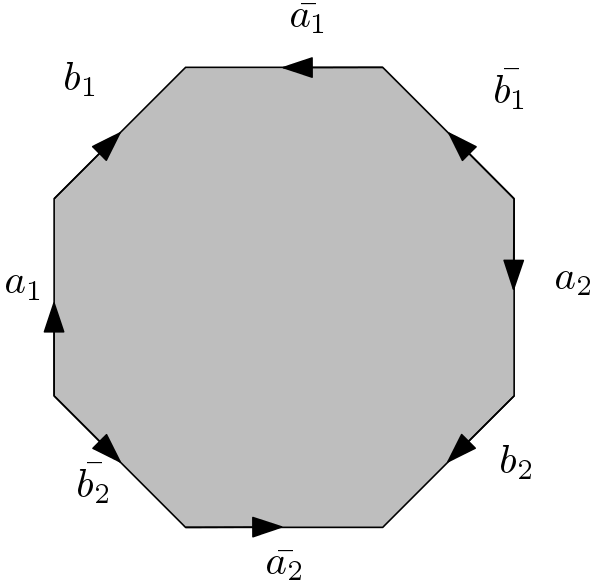
\includegraphics[scale=0.2]{imatesis.png}
\end{center}

In general, this decomposition gives the following presentation of the fundamental group of $\Sigma$:
\[\pi_1(\Sigma)=\bigg{\langle} a_1,\dots, a_g, b_1, \dots, b_g \quad | \quad \prod_{i=1}^g [a_i,b_i]=1 \bigg{\rangle}, \]
here $[a,b]$ denotes the commutator $aba^{-1}b^{-1}$. Thus, a representation $\rho$ of $\pi_1(\Sigma)$ on $G$ is the same as a choice of matrices
$A_1,\dots,A_g,B_1, \dots B_g \in G$ such that \[\prod_{i=1}^g [A_i,B_i]=\id.\]
We have seen that such a representation gives rise to a vector bundle $E^\rho$ and the natural question arises of computing the degree of $E^\rho$ in terms of
the matrices $A_i, B_i$.


Let $\tilde{G}$ be the universal cover of $G$ and consider the short exact sequence  
\[0 \rightarrow \pi_1(G) \xrightarrow{\iota} \tilde{G} \xrightarrow{p} G \rightarrow 0.\]

Consider also the map $\phi: \R \rightarrow S$ given by:

$$\begin{array}{rcc}
\alpha & \longmapsto & \left[ {\begin{array}{cc}
	\cos \alpha & \sin \alpha\\
	-\sin \alpha & \cos \alpha \\
	\end{array} }  \right] .
\end{array}$$

The map $\phi$ is the universal covering map of $S$ and therefore the retraction map $\theta: G \rightarrow S$ can be lifts naturally to a map:
\[ \hat{\theta}: \tilde{G} \rightarrow \R.\]

Thus we obtain the following commutative diagram:
\begin{center}
	\begin{tikzcd}
		& 0 \arrow[d] & 0 \arrow[d] &  \\
		& \pi_1(G) \arrow[r] \arrow[d,"\iota"] & \mathbb{Z} \arrow[d, "2 \pi"] & \\
		& \tilde{G} \arrow[r, "\tilde{\theta}"] \arrow[d,"p"] & \mathbb{R}  \arrow[d,"\phi"] &\\
		\pi_1(\Sigma) \arrow [r, "\rho"]	&G \arrow[r,"\theta"]  & S &
	\end{tikzcd}	
\end{center}


\begin{lemma}
	Given a homomorphism $\rho: \pi_1(\Sigma) \rightarrow G$ determined by matrices $A_1, \dots, A_g, B_1,\dots, B_g$ we define the number $\delta(\rho)$ by:
	\[ \delta(\rho):= \frac{1}{2\pi}\tilde{\theta}(\prod_{i=1}^g [\alpha_i,\beta_i])\in \mathbb{Z}.\]
	Here $\alpha_i, \beta_i$ are elements in $\tilde{G}$ such that $p(\alpha_i)=A_i$ and $p(\beta_i)=B_i$. This number depends only on $\rho$.
\end{lemma}
\begin{proof}
	Let us first proof that for any choice of the $\alpha_i$ and $\beta_i$ the number $\delta(\rho)$ is an integer. By construction, $\prod_{i=1}^g [\alpha_i,\beta_i] \in \mathsf{ker}(p)$. This implies that $\hat{\theta}(\prod_{i=1}^g [\alpha_i,\beta_i])$ is a multiple of $2\pi$ and the result follows. Let us now show that the number is well defined. Suppose that $\alpha_i'$ and $\beta_i'$ is a different choice. Then, for each $i$ we know that:
	\[ \alpha_i'=\alpha_i x_i\;\, \beta_i'= \beta_i y_i ,\]
	where the $x_i$ and the $y_i$ are in the kernel of $p$ which is contained in the center of $\tilde{G}$. This implies that:
	\[ [\alpha_i, \beta_i]=[\alpha_i',\beta_i'],\]
	and the result follows.
\end{proof}
\begin{lemma}
	Given a representation $\rho: \pi_1(\Sigma) \rightarrow G$ we have:
	\[ \delta(\rho)=D(E^\rho).\]
\end{lemma}

\begin{proof}
	This will be added later.
\end{proof}

\begin{exercise}\label{trace}
	Show that if
	\[A= \left( {\begin{array}{cc}
		a & b\\
		c & d \\
		\end{array} } \right) \in G,\] then 
	\[\theta(A)=\frac{1}{\sqrt{x^{2}+y^{2}} } \left( {\begin{array}{cc}
		x & y\\
		-y &  x \\
		\end{array} } \right). \]
	Here $x=a+d$ and $y=b-c$.
	Moreover, show that:			
	\begin{enumerate}
		\item If $A \in G$ has positive trace, then $\theta(A)$ has positive trace.
		\item If $A$ and $B$ are symmetric and positive definite matrices, then $AB$ has positive trace.
		\item If $A,B \in G$ are symmetric and positive definite matrices, then $\theta(A B)$ has positive trace.
		\item $\theta(A^{-1})=\theta(A)^{-1}$.
	\end{enumerate}
\end{exercise}




\begin{lemma}\label{angle}
	The function $\tilde{\theta}: \tilde{G} \to \mathbb{R} $ satisfies the property:
	\[|\tilde{\theta}(\alpha \beta)-\tilde{\theta}(\alpha)-\tilde{\theta}(\beta)|<\pi/2.\]
\end{lemma}
\begin{proof}
	Given $A,B\in G$, then there exists symmetric positive definite matrices $R,T$ such that:  	
	\[AB=\theta(A)R \theta(B)T.\]
	If we set $X=\theta(B)^{-1}R\theta(B)$ then:
	\[AB=\theta(A)\theta(B)XT.\]
	This implies that: \[\theta(AB)=\theta(A)\theta(B)\theta(XT).\] 
	Therefore:
	\[\theta(B)^{-1}\theta(A)^{-1}\theta(AB)=\theta(XT) .\]
	Since $X,T$ are positive definite, the previous Exercise \ref{trace} implies that $\theta(B)^{-1}\theta(A)^{-1}\theta(AB)$ has positive trace.
	Fix $\alpha, \beta \in \tilde{G}$ such that $p(\alpha)=A$ and $p(\beta)=B$ and 
	set $\Delta=\tilde{\theta}(\alpha \beta)-\tilde{\theta}(\alpha)-\tilde{\theta}(\beta)$. Then:
	\[ \phi(\Delta)=\left[ {\begin{array}{cc}
		\cos \Delta & \sin \Delta \\
		-\sin \Delta & \cos \Delta \\
		\end{array} } \right]=\theta(B)^{-1}\theta(A)^{-1}\theta(AB)\]
	has positive trace. So $cos \Delta >0$. Since $\Delta$ is a continuous function of $\alpha$ and $\beta$ which vanishes when $\alpha=\beta=1$ we conclude that
	$|\Delta|<\frac{\pi}{2}$.
	
	
\end{proof}


\begin{lemma}\label{bound}
	Given a representation $\rho: \pi_1(\Sigma) \rightarrow G$ we have:
	\[ |\delta(\rho)|<g.\]
\end{lemma}

\begin{proof}
	Applying Lemma \ref{angle} $4g-1$ times one obtains:
	\[|\tilde{\theta}([\alpha_1,\beta_1]\dots [\alpha_g,\beta_g] )-\tilde{\theta}(\alpha_{1})-\tilde{\theta}(\beta_{1})-\tilde{\theta}(\alpha_{1}^{-1})-\tilde{\theta}(\beta^{-1}_1) \dots-\tilde{\theta}(\alpha_{g})-\tilde{\theta}(\beta_{g})-\tilde{\theta}(\alpha_{g}^{-1})-\tilde{\theta}(\beta^{-1}_g)  | \]
 	 \[	<(4g-1)\frac{\pi}{2}\] 
	By Exercise \ref{trace} we know that 
	\[\tilde{\theta}(\alpha)+\tilde{\theta}(\alpha^{-1})=0,\]
	so that the inequality above becomes:
	\[|\tilde{\theta}([\alpha_1,\beta_1]\dots [\alpha_g,\beta_g])  |<(4g-1)\frac{\pi}{2}.\]
	
	Dividing by $2\pi$ one obtains:
	\[ |\delta(\rho)|<g-\frac{1}{4}<g.\]
	
\end{proof}

The lemma gives one direction of Milnor's inequalities. We will now show that the converse is also true.

\begin{exercise}\label{center}
	Let $G$ be a connected Lie group with universal cover $\tilde{G}$. Show that if $g \in \tilde{G}$ is such that $p(g) \in Z(G)$ then $g \in Z(\tilde{G})$.
\end{exercise}





Let us set $A_{0}:= \left( \begin{array}{cl} 
2 & 0 \\
0 & 1/2
\end{array} \right)  $                    and   $\alpha_{0} \in p^{-1}(A_{0})$ so that $\tilde{\theta}(\alpha_{0})=0$.
We will denote by $K$ and $\tilde{K}$ the conjugacy classes of $A_{0}$ and $\alpha_{0}$ respectively. \\

Since $\R$ is simply connected, the group homomorphism $\phi: \R \rightarrow G$ lifts to a homomorphism $\R \rightarrow \tilde{G}$ and therefore
$\R$ acts on $\tilde{G}$ and also on conjugacy classes of $\tilde{G}$.





\begin{lemma}\label{product}
	Any element of $\pi \tilde{K}$ can be written as a product of two elements in $\tilde{K}$.
\end{lemma}
\begin{proof}
	Consider the matrices:
	
	\[A_{1}=\left(  \begin{array}{cl}
	-5/2 & 9/2\\
	-3 & 5
	\end{array}\right)\] and 
	\[A_{2}=A_{0} A_{1} =
	\left( \begin{array}{cl}
	-5 & 9\\
	-3/2 & 5/2
	
	\end{array}\right).\]
	
	Since the trace and determinant characterise the sets ${K}$ and $ \pi K$,
	then $A_{0}, A_{1} \in K$ and  $A_{2} \in \pi K$.
	Let  $\alpha_{0},\alpha_{1} \in \tilde{K} $ be such that $p(\alpha_i)=A_i$ and $\tilde{\theta}(\alpha_{i})=0$. Then $\alpha_{0} \alpha_{1} \in  n\pi \tilde{K}$ for some odd integer $n$. Let us show that $n=\pm1$.
	Given  $\alpha \in \tilde{K}$ we know that $p(\alpha)$ has positive trace and therefore $\cos(\tilde{\theta}(\alpha))>0$.
	Therefore, if $\beta \in n\pi \tilde{K}$ with $|n|>1$ then:
	
	\[|\tilde{\theta}(\beta)|>\frac{5\pi}{2}.\]
	Applying Lemma \ref{angle} we obtain:
	
	\[ |\tilde{\theta}(\alpha_{0} \alpha_{1})|< |\tilde{\theta}(\alpha_{0})|+|\tilde{\theta}(\alpha_{1})| + \frac{\pi}{2} < \frac{3}{2} \pi \]
	
	We conclude that $n=\pm1$.
	\begin{itemize}
		\item If $n=1$ we set:\[\gamma(\alpha_{0} \alpha_{1})\gamma^{-1}=(\gamma \alpha_{0} \gamma^{-1})(\gamma \alpha_{1} \gamma^{-1}) \in \tilde{K}\tilde{K}.\]
		\item If $n=-1$ then $\gamma(\alpha_{0} \alpha_{1})\gamma^{-1} \in -\pi \tilde{K}$ and $\gamma(\alpha_{0} \alpha_{1})^{-1} \gamma^{-1} \in \pi \tilde{K}$. We then write:
		\[\gamma(\alpha_{0} \alpha_{1})^{-1}\gamma^{-1}=(\gamma \alpha_{1}^{-1} \gamma^{-1})(\gamma \alpha_{0}^{-1}\gamma^{-1}) \in \tilde{K} \tilde{K}.\]
	\end{itemize}
\end{proof}

\begin{lemma}\label{lema_3}
	For every $\alpha \in \pi \tilde{K}$ there exists $\beta_1 \beta_{2} \in \tilde{G}$ so that $\alpha=\beta_{1}\beta_{2}\beta_{1}^{-1}\beta_{2}^{-1}$.
\end{lemma}
\begin{proof}
	By the previous lemma there exists $\beta_{1},\beta_{3} \in \tilde{K}$ so that $\alpha=\beta_{1}\beta_{3}$. Since $\alpha_{1} ^{-1} \in \tilde{K}$ there exists $\beta_{2} \in \tilde{G}$ so that $\beta_{2} \alpha_{1}^{-1} \beta_{2}^{-1}=\beta_{3}$.\\
	Then $$\alpha=\beta_{1} \beta_{3}=\beta_{1} \beta_{2} \beta_{1}^{-1}\beta_{2}^{-1}$$
\end{proof}
\begin{lemma}\label{list}
	For every $n \geq1 $ there exists $\gamma_1,\dots, \gamma_{n+1} \in \tilde{K}$ so that $\gamma_1 \dots \gamma_{n+1}=n \pi\alpha_{0}.$
\end{lemma}
\begin{proof}
	We will argue by induction. The case $n=1$ is Lemma \ref{product}. Now assume that the lemma holds for $n$ so that we can write:
	\[\gamma_1 \dots \gamma_{n+1}=n \pi\alpha_{0}.\] Then:
	
	\[ (n+1)\pi \alpha_0= \pi (n \pi) \alpha_0=\pi (\gamma_1 \dots \gamma_{n+1})=(\pi \gamma_1) \dots \gamma_{n+1}=\gamma \gamma' \gamma_2 \dots \gamma_{n+1}.\]
	Here $\gamma, \gamma' \in \tilde{K}$ and we have applied the Lemma product to $\pi \gamma_1$.
	
\end{proof}





\begin{theorem}\label{Milnor}
	A rank two oriented vector bundle $\pi:E \rightarrow \Sigma$ admits a flat connection if and only if:
	\[ |D(E)|<g.\]
\end{theorem}

\begin{proof}
	One direction is guaranteed by Lemma \ref{bound}. We want to prove that a bundle $E$ with $|D(E)|<g$ admits a flat connection. It suffices to show that
	there is some representation $\rho: \pi_1(\Sigma) \rightarrow G$ such that $\delta(\rho)=D(E)$. Since the existence of a flat connection does not depend on the orientation we may assume that $D(E)>0$. Since some of the matrices in the representation can be set to $\id$ it suffices to show the case where $D(E)=g-1$ and $g>1$.
	By Lemma \ref{list} there exist $\gamma_{1},...,\gamma_{g-1} \in \tilde{K}$ so that:
	\[\gamma_1 \dots \gamma_{g-1}=(g-2) \pi\alpha_{0}.\]
	
	If we set $\gamma_g=\alpha_{0}^{-1}$ then:
	\[\gamma_1 \dots \gamma_{g-1}\gamma_g=(g-2) \pi.\]
	
	Now by Lemma \ref{lema_3}, for every $1 \leqslant i \leqslant g$ there exists $\alpha_i,\beta_i \in \tilde{G}$ so that 
	\[[\alpha_i,\beta_i]= \pi \gamma_i.\]
	Then 
	\[\prod_{i=1}^g[\alpha_i,\beta_i]=2\pi (g-1).\]
	
	This implies that by setting $A_i=p(\alpha_i)$ and $B_i=p(\beta_i)$ one obtains a representation $\rho$ such that:
	\[\delta(\rho)=\frac{1}{2\pi}\prod_{i=1}^g[\alpha_i,\beta_i]= g-1.\]
\end{proof}


\begin{corollary}
	The torus is the only closed oriented surface that admits an affine structure. In particular, Chern's conjecture holds in dimension $d=2$.
\end{corollary}
\begin{proof}
	Since $S^2$ is simply connected, a flat connection on $TM$ would give a trivialization of $TM$, which does not exist because the Euler characteristic of the sphere is $2$.
	Let us now assume that $g>1$. Then $D(TM)=\chi(\Sigma)=2-2g$. Then:
	\[|D(TM)|= 2|(1-g)|=2g-2 \geq g.\]
\end{proof}
